
\chapter{The market forces and supply and demand}

Supply and demand are the two words that economists use most often --- and for good reasobn.
Supply and demand are the forces that make market economies work.
They determine the quantity of each good produced and the price at which it is sold.
If you want to know how any event or policy will affect the economy, you must think first about how it will affect supply and demand.


\section{Market and compition}

The terms supply and demand refer to the behavior of people as they interact with one another in markets.
A market is a group of buyers and sellers of a particular good or service.
The buyers as a group determine the demand for the product, and the sellers as a group determine the supply of the product.



\subsection{Competitive markets}

A competitive market is a market in which there are many buyers and many sellers so that each has a negligible impact on the market price.


\subsection{Competition: perfect and otherwise}

We assume the market is perfectly competitive for study.
Perfectly competitive market are defined by two primary characteristics:
\begin{enumerate}
\item the goods being offered for sale are all the same 
\item the buyers and sellers are so numerous that no single buyer or seller can influence the market price.
\end{enumerate}
Because buyers and sellers in perfectly competitive markets must accept the price the market determines, they are said to be \keyword{price takers}.


Not all goods and services, however, are sold in perfectly competitive markets.
Some markets have only one seller, and this seller sets the price.
Such a seller is called a \keyword{monopoly}.


Some markets fall between the extremes of perfect competition and monopoly.
One such market, called an \keyword{oligopoly}, has a few sellers that do not always compete aggressively. 
Airline routes are an example.
If a route between two cities is serviced by only two or three carriers, the carriers may avoid rigorous competition to keep prices high.
Another type of market is \keyword{monopolistically competitive}; it contains many sellers, each offering a slightly different product.
Because the products are not exactly the same, each seller has some ability to set the price for its own product.
An example is the software industry.
Many word processing programs compete with one another for users, but every program is different from every other and has its own price.



\section{Demand}

\begin{tcolorbox}
\keyword{quantity demand: the amout of a good that byers are willing and able to purchase.}  
\end{tcolorbox}

\subsection{What determines the quantity an individual demands?}

\subsubsection{Price}

\keyword{law of demand:}
Other things equal, when the price of a good rises, the quantity demanded of the good falls.


\subsubsection{Income}

If the demand for a good falls when income falls, the good is called a \keyword{normal good}.
If the demand for a good rises when income falls, the good is called an \keyword{inferior good.}


\subsubsection{Price of related goods}

When a fall in the price of one good reduces the demand for another good, the two goods are called \keyword{substitutes}.
When a fall in the price of one good raises the demand for another good, the two goods are called complements.

\subsubsection{Tastes}

The most obvious determinant of your demand is your tastes.
Economists normally do not try to explain people’s tastes because tastes are based on historical and psychological forces that are beyond the realm of economics.
Economists do, however, examine what happens when tastes change.


\subsubsection{Expectations}

Your expectations about the future may affect your demand for a good or service today.


\subsection{The demand schedule and the demand curve}

Imagine that we hold all these variables constant except one --- the price.
Let’s consider how the price affects the quantity of ice cream demanded.

\begin{figure}[!ht]
  \centering
  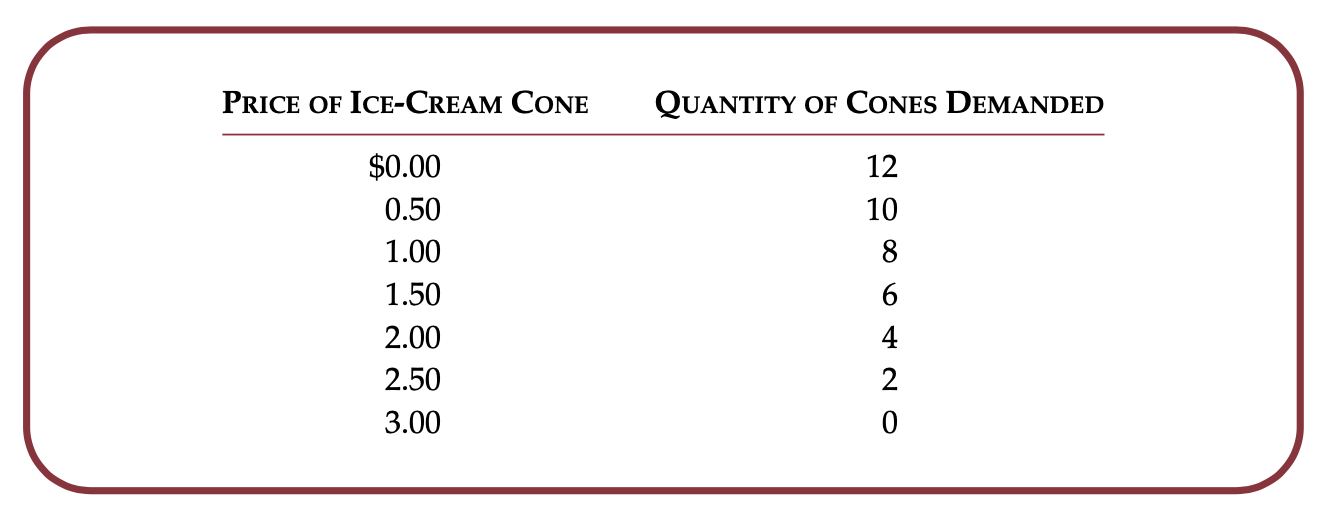
\includegraphics[width=\textwidth]{pics/demand-schedule}
  \caption{Demand schedule}
  \label{fig:demand-schedule}
\end{figure}

\begin{figure}[!ht]
  \centering
  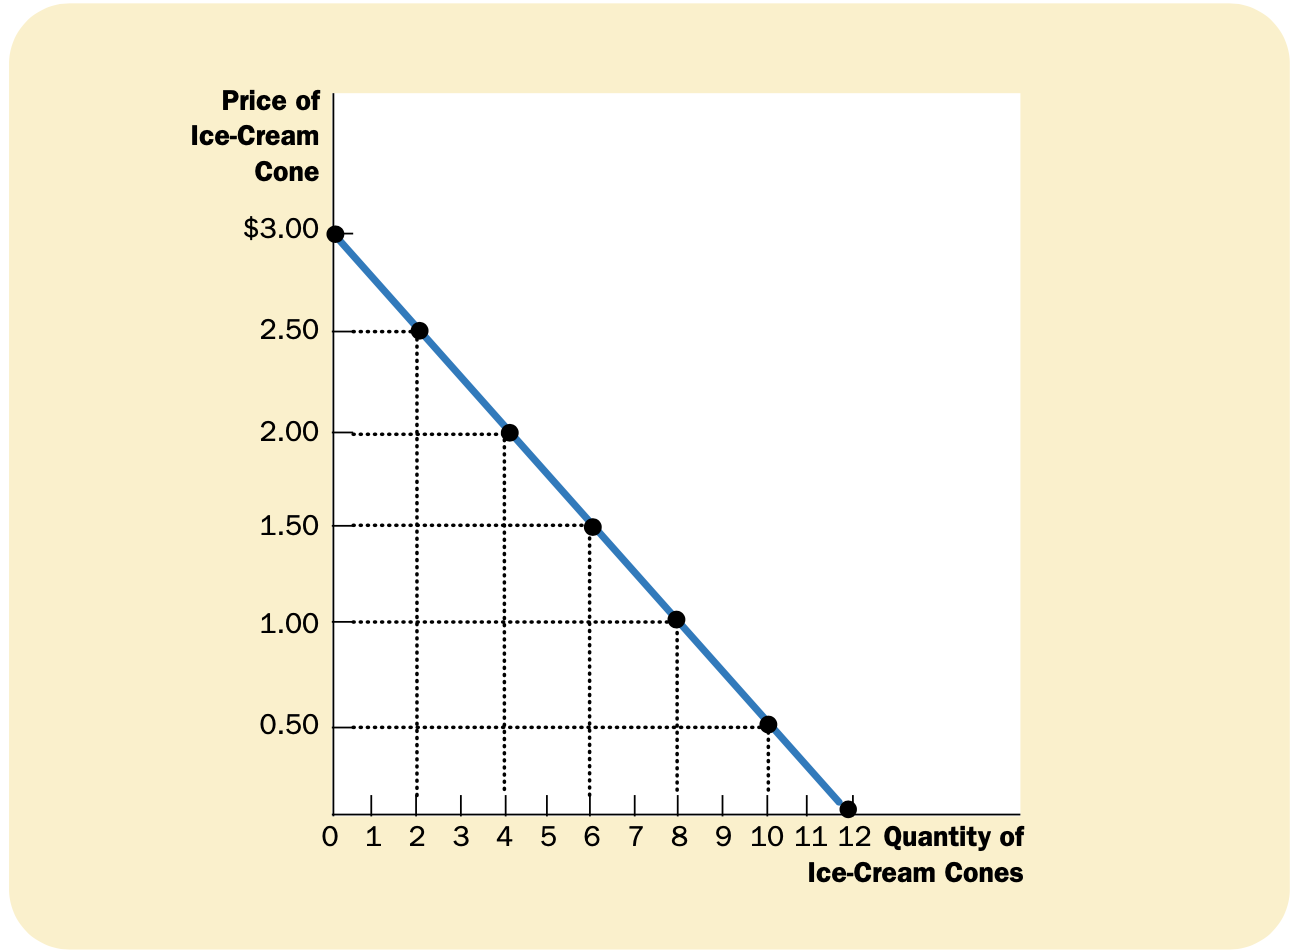
\includegraphics[width=\textwidth]{pics/demand-curve}
  \caption{Demand curve}
  \label{fig:demand-curve}
\end{figure}

Table \ref{fig:demand-schedule} is a \keyword{demand schedule}, able that shows the relationship between the price of a good and the quantity demanded.
Figure \ref{fig:demand-curve} graphs the numbers in Table \ref{fig:demand-schedule}.
By convention, the price of ice cream is on the vertical axis, and the quantity of ice cream demanded is on the horizontal axis.
The downward-sloping line relating price and quantity demanded is called the \keyword{demand curve}.

\subsection{Ceteris paribus}

Economists use the term \keyword{ceteris paribus} to signify that all the relevant variables, except those being studied at that moment, are held constant.
The Latin phrase literally means ``other things being equal.''
The demand curve slopes downward because, ceteris paribus, lower prices mean a greater quantity demanded.


\subsection{Market demand versus individual demand}

To analyze how markets work, we need to determine the \keyword{market demand}, which is the sum of all the individual demands for a particular good or service.

\subsection{Shift in the demand curve}



Whenever any determinant of demand changes, other than the good's price, the demand curve shifts.
As Figure \ref{fig:shift-in-demand-curve} shows, any change that increases the quan- tity demanded at every price shifts the demand curve to the right.
Similarly, any change that reduces the quantity demanded at every price shifts the demand curve to the left.

\begin{figure}[!ht]
  \centering
  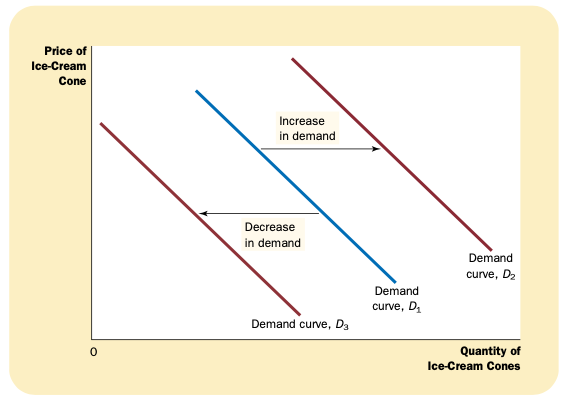
\includegraphics[width=\textwidth]{pics/shift-in-demand-curve}
  \caption{Shift in demand curve}
  \label{fig:shift-in-demand-curve}
\end{figure}

\begin{tcolorbox}
  The demand curve shows what happens to the quantity demanded of a good when its price varies, holding constant all other determinants of quantity demanded.
  When one of these other determinants changes, the demand curve shifts.
\end{tcolorbox}

\section{Supply}

The \keyword{quantity supplied} of any goods or services is the amount that sellers are willing and able to sell.


\subsection{What determine the quantity an individual supplies?}

\subsubsection{Price}

\keyword{law of supply}:
Other things equal, when the price of a good rises, the quantity supplied of the good also rises.


\subsubsection{Input prices}

The supply of a good is negatively related to the price of the inputs used to make the good.


\subsubsection{Technology}

The advance in technology raised the supply.


\subsubsection{Expections}

The amount of goods or services you supply today may depend on your expectations of the future.


\subsection{The supply schedule and the supply curve}

\begin{figure}[!ht]
  \centering
  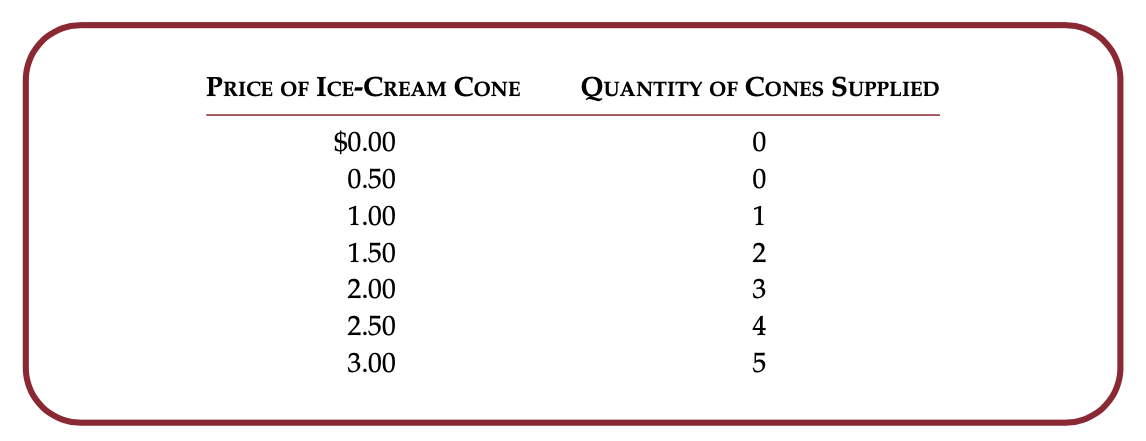
\includegraphics[width=\textwidth]{pics/supply-schedule}
  \caption{Supply schedule}
  \label{fig:supply-schedule}
\end{figure}


\begin{figure}[!ht]
  \centering
  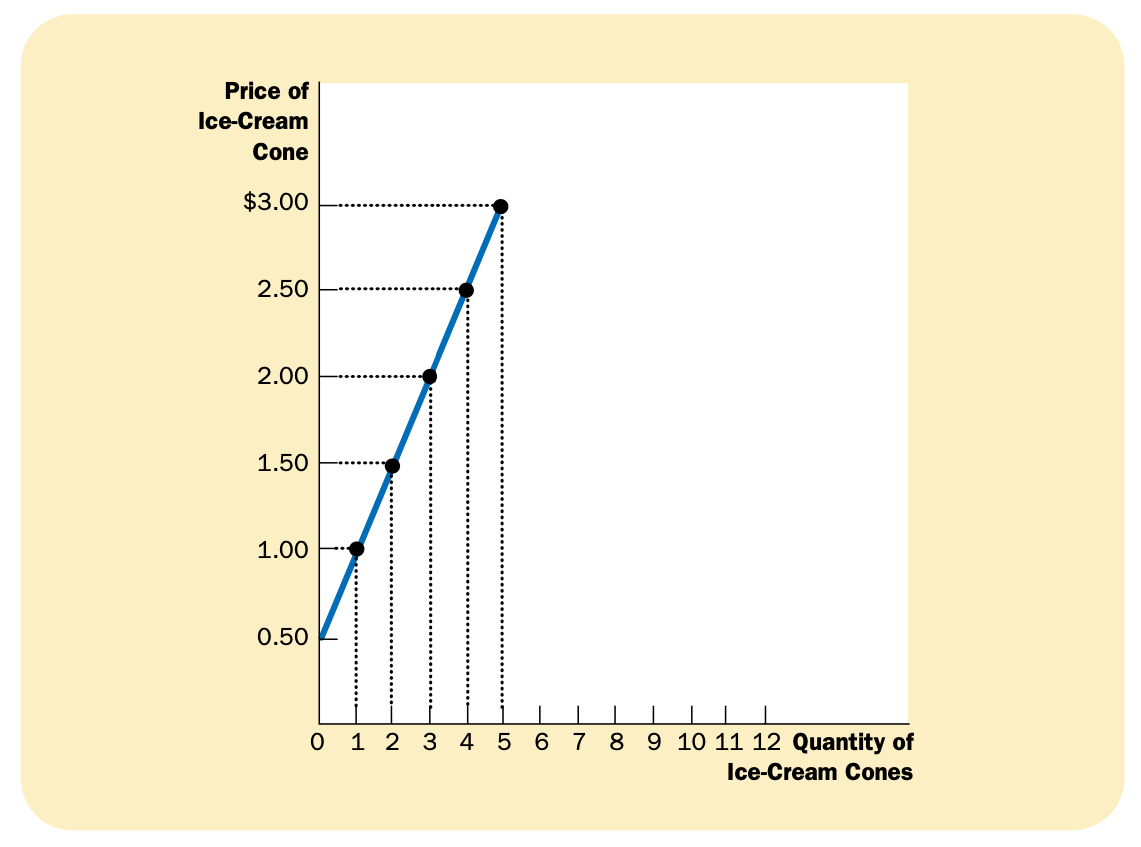
\includegraphics[width=\textwidth]{pics/supply-curve}
  \caption{Supply curve}
  \label{fig:supply-curve}
\end{figure}

Table \ref{fig:supply-schedule} is called the \keyword{supply schedule}.
Figure  \ref{fig:supply-curve} is called the \keyword{supply curve}.


\subsection{Market supply vs individual supply}

Market supply is the sum of the supplies of all sellers.


\subsection{Shifts in the supply curve}

Whenever there is a change in any determinant of supply, other than the good’s price, the supply curve shifts.
As Figure \ref{fig:shifts-in-the-supply-curve} shows, any change that raises quantity supplied at every price shifts the supply curve to the right.
Similarly, any change that reduces the quantity supplied at every price shifts the supply curve to the left.


\begin{figure}[!ht]
  \centering
  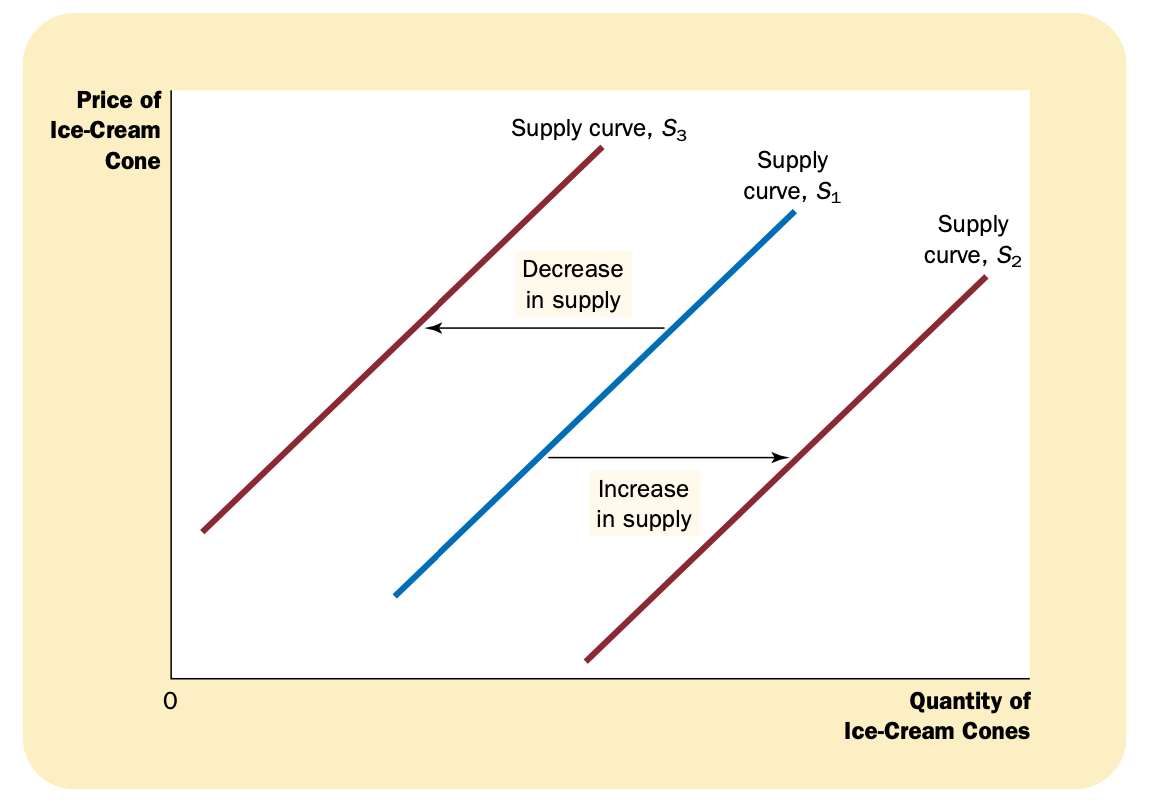
\includegraphics[width=\textwidth]{pics/shifts-in-the-supply-curve}
  \caption{Shifts in the supply curve}
  \label{fig:shifts-in-the-supply-curve}
\end{figure}


The supply curve shows what happens to the quantity supplied of a good when its price varies, holding constant all other determinants of quantity supplied.
When one of these other determinants changes, the supply curve shifts.




\section{Supply and demand together}

\begin{figure}[!ht]
  \centering
  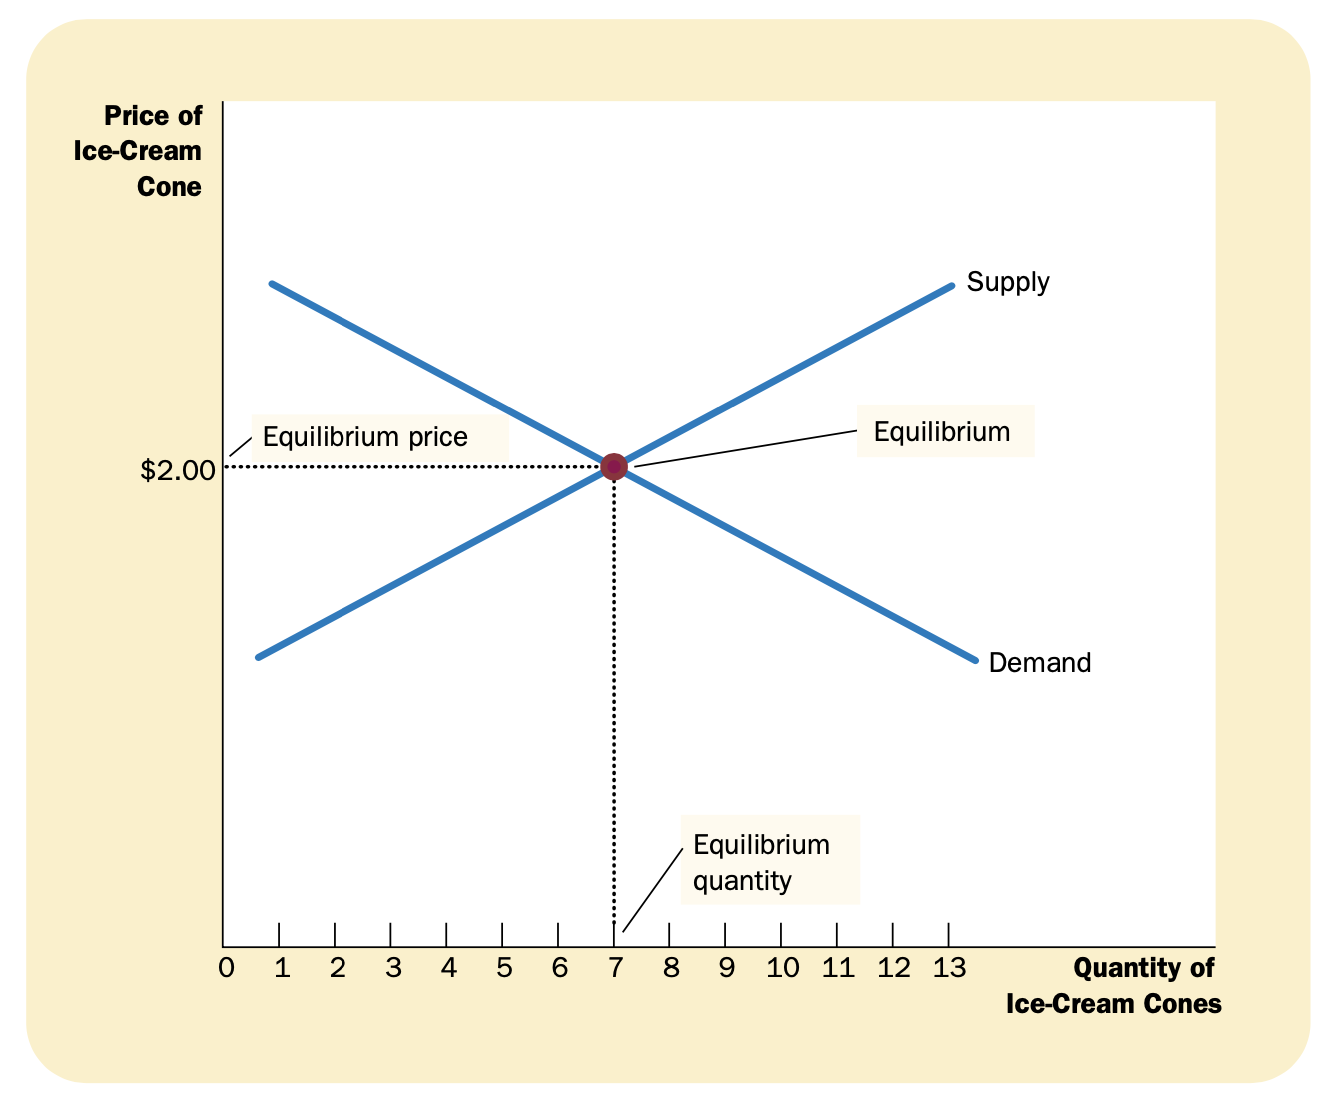
\includegraphics[width=\textwidth]{pics/equilibrium-of-supply-and-demand}
  \caption{The equilibrium of supply and demand}
  \label{fig:the-equilibrium-of-supply-and-demand}
\end{figure}

\ref{fig:the-equilibrium-of-supply-and-demand} shows the market supply curve and market demand curve together.
There is one point at which the supply and demand curves intersect;
this point is called the market's \keyword{equilibrium}.
The price at which these two curves cross is called the \keyword{equilibrium price}, and
the quantity is called the \keyword{equilibrium quantity}.


The dictionary defines the word equilibrium as a situation in which various forces are in balance—and this also describes a market’s equilibrium.
At the equilibrium price, the quantity of the good that buyers are willing and able to exactly balances the quantity that sellers are willing and able to sell.
The equilibrium price is sometimes called the \keyword{market-clearing price} because, at this price, everyone in the market has been satisfied: Buyers have bought all they want to buy, and sellers have sold all they want to sell.


The actions of buyers and sellers naturally move markets toward the equilibrium of supply and demand.

\begin{figure}[!ht]
  \centering
  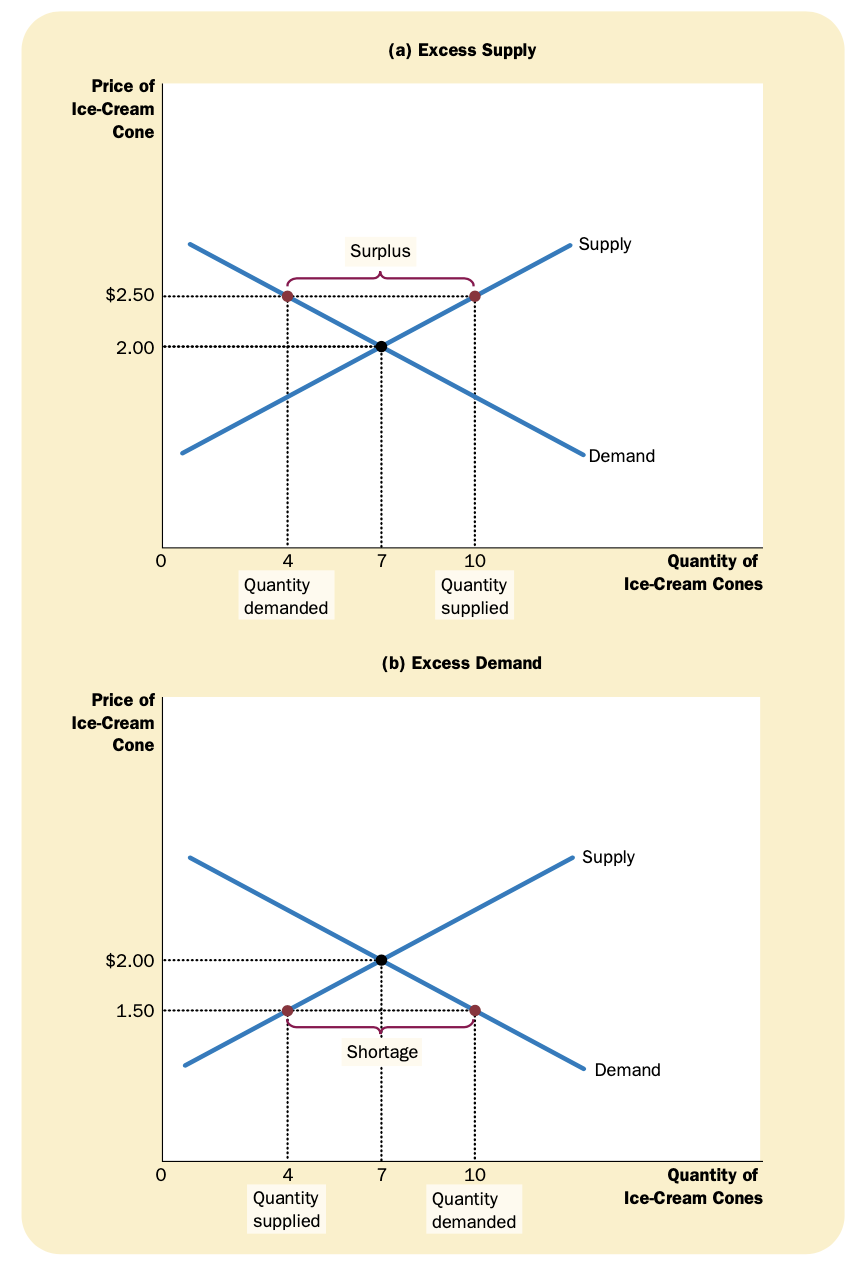
\includegraphics{pics/surplus-and-shortage}
  \caption{Surplus and shortage}
  \label{fig:surplus-and-shortage}
\end{figure}


\keyword{surplus}:
a situation in which quantity supplied is greater than quantity demand.

\keyword{shortage}:
a situation in which quantity demand is greater than quantity supplied.

\keyword{law of supply and demand}:
The price of any good adjusts to bring the supply and demand for that good into balance.

\subsection{Three steps to analyzing changes in equilibrium}

The equilibrium price and quantity depend on the position of the supply and demand curves.
When some event shifts one of these curves, the equilibrium in the market changes.
The analysis of such a change is called \keyword{comparative statics}
because it involves comparing two static situations --- an old and a new equilibrium.


When analyzing how some event affects a market, we proceed in three steps:
\begin{tcolorbox}
\begin{enumerate}
\item Decide whether the event shifts the supply curve or demand curve (or perhaps both).
\item Decide which direction the curve shifts.
\item Use the supply-and-demand diagram to see how the shift changes the equilibrium
\end{enumerate}  
\end{tcolorbox}


